\section*{Problem 6}

\subsection*{Part 1}
$$
\begin{array}{l}
\dot{x}_{1}=x_{1}^{3}+x_{1}^{2} x_{2} \\
\dot{x}_{2}=-x_{2}+x_{2}^{2}+x_{1} x_{2}-x_{1}^{3}
\end{array}
$$

\noindent In order to show that the given system is unstable, according the Lyapunov Stability Theorem, it is sufficient to show that conditions for stability do not hold in the domain about the origin. This can be seen computing the time derivate of the Lyapunov function and substituting in the state equations.
$$
V=x_{1}\left(x_{1}^{3}+x_{1}^{2} x_{2}\right)+x_{2}\left(-x_{2}+x_{2}^{2}+x_{1} x_{2}-x_{1}^{3}\right)
$$

\noindent Given this formulation, we know that according to Lyapunov's stability theorem that the function must be negative semi definite for the system to be stable. Under this condition, the previous equations simplifies to the following expression.

$$
x_{1}^{4}-x_{2}^{2}+x_{2}^{3}+x_{1} x_{2}^{2} \leq 0
$$

\noindent Since it is rather difficult to analytically show the regions where this inequality holds, we can show numerically that there does not since exist a neighborhood around the origin, such that the ball $B_r = \{ x \in D \subset \R^2 | \left\Vert x \right\Vert < r \}$ maintains the previous inequality. This is the case for point $x = (.5, .5)$ for $r <1$. When evaluated at this point the inequality does not hold. Since we cannot define a ball around the origin such that the equality holds for \textbf{all} points contained inside of that ball, we must conclude that the system is \underline{unstable}.  In particular, I believe that the points in the 1st quadrant of the of statespace do not hold for the inequality.

\subsection*{Part 2}


$$
\begin{array}{l}
\dot{x}_{1}=-x_{1}^{3}+x_{2} \\
\dot{x}_{2}=x_{1}^{6}-x_{2}^{3}
\end{array}
$$


In the problem statement, we are told to investigate the set defined by $\Gamma=\left\{0 \leq x_{1} \leq 1\right\} \cap\left\{x_{2} \geq x_{1}^{3}\right\} \cap\left\{x_{2} \leq x_{1}^{2}\right\}$, which would give us insight into the stability of the system. We can graphically show this set by plotting the two curves over the valid domain shown. The area between these curves represented the graphical description of the set $\Gamma$. \\


\begin{center}
  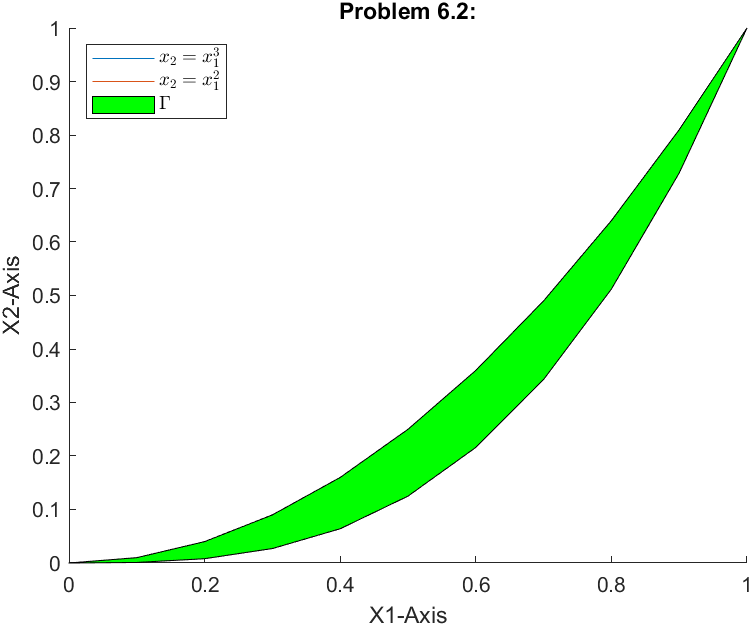
\includegraphics[scale=.75]{Gamma_6_2}
\end{center}



\noindent By investigating the behavior of the functions at both of its borders, we can develope an intuitiion about the behavior of the system and whether the origin is stable or not. We can accomplish this by setting each state equation independently to $0$ and determining the behavior of the remaining component of the trajectory; however, since we know that the set $\Gamma$ is an invariant set, we know that any trajectory started inside of this set will remain in this set, can investigate the stability of the origin, but observing how trajectories behave. We can visualize this behavior numerically by looking at the vector field of the problem and noticing that even initial conditions very close to the origin, diverge away from it and converge to the point (1,1), as shown in the figure below.


\begin{center}
  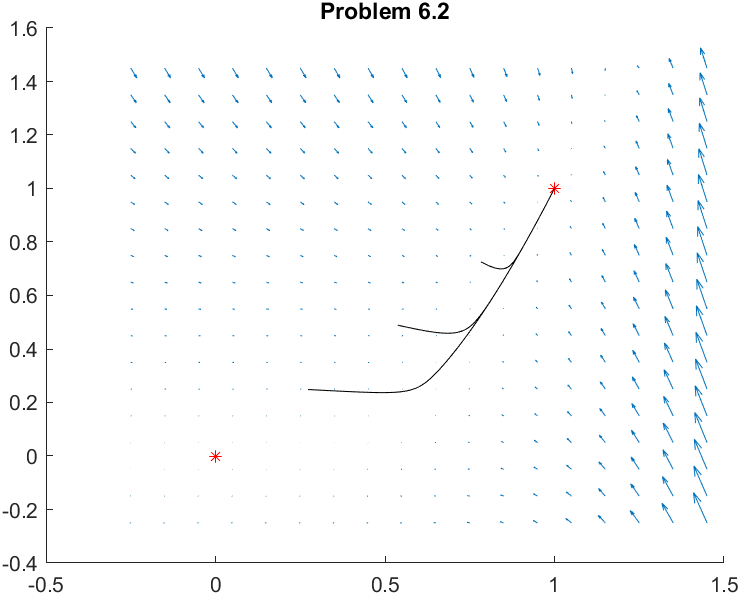
\includegraphics[scale=.75]{6_2_vector_Field}
\end{center}


\noindent However, we can show this same behavior analytically such that ...

$$
\dot{x}_2 = 0 \rightarrow  \dot{x}_1 > 0
$$

\noindent Similarly...

$$
\dot{x}_1 = 0 \rightarrow \dot{x}_2 > 0
$$

\noindent This means any tracjectory starting inside of $\Gamma$, the values of $x_1$ and $x_2$ will continue to increase, unless the system is already at an equilibirum point. However, if the trajectory is not begun at an equilibrium point, then the value of the trajectory will continue to grow, until it reaches $x =1$. This means that the origin of the system is \underline{unstable}, since the only valid values of the system are greater than $x=0$, and since the trajectory will only increase in value over time, there does not exist any point (other than $x=0$), which will converge to the origin.

 
